\documentclass[12pt,oneside,final]{ucthesis}

\includeonly{%
  abstract,
  introduction,
  methods,
  results,
  discussion,
  conclusions,
  appendix
}
% from ucthesis
\usepackage{amssymb}
\usepackage{multirow}
\usepackage{amsthm}

% enable epigraphs
\usepackage{epigraph}
\renewcommand{\textflush}{flushepinormal}

% enable text super- and sub- scripts
\usepackage{xltxtra}
\usepackage{caption}
% let us typeset things inside the captions
\captionsetup{justification=justified}

\usepackage{graphicx}
% used for pmatrix
\usepackage{amsmath}
\usepackage{array}

\usepackage{inconsolata}

% short space lists
\usepackage{enumitem}
\setlist{nolistsep}

% have a table that spans two pages...
\usepackage{longtable}

\usepackage[sc,osf]{mathpazo}
\usepackage[T1]{fontenc}
%\usepackage{inconsolata}

% use fancy syntax highlighting provided by an interface to pygments
\usepackage{minted}

%\usepackage[margin=.75in,nohead,nofoot]{geometry}⋅
%\usepackage[nohead]{geometry}
\usepackage{hyperref}
\usepackage[authoryear,round]{natbib}

% named colors, package already included with minted
\definecolor{DBlue}{rgb}{0.19,0.32,0.50}
\definecolor{DRed}{rgb}{0.7,0.22,0.21}
\definecolor{DGreen}{rgb}{0.15,0.41,0.15}
\definecolor{LGreen}{rgb}{0.01,0.62,0}

%\setlength{\parskip}{0.05in}
%\linespread{1.2}

\def\newblock{\hskip .11em plus .33em minus .07sem}

\hypersetup{
  colorlinks = true,
  urlcolor = black,
  citecolor = blue
}

\renewcommand{\theFancyVerbLine}{\sffamily\textcolor[rgb]{0.5,0.5,0.5}{\scriptsize\arabic{FancyVerbLine}}}

\begin{document}
  \title{\Huge{Assessing ship movements using volunteered geographic information}}
  \author{Shaun Walbridge}

  \report{Thesis}
  \degree{Master of Arts}
  \degreemonth{March}
  \degreeyear{2013}
  \approvalmonth{December}
  \approvalyear{2012}

  \chair{Professor Steven D. Gaines}
  \committeeII{Research Professor Robert R. Warner}
  \committeeIII{Assistant Professor Krzysztof W. Janowicz}
  \nummembers{3}
  \field{Ecology, Evolution, and Marine Biology}
  \campus{Santa Barbara}

\maketitle{}

\begin{frontmatter}
    %% Template pages
  \approvalpage 
  \copyrightpage

  %% Dedication
%   \begin{dedication}
%     \null\vfil{%\large
%       \hspace{\stretch{1}}
%       \begin{minipage}{3.2in}
%         \begin{center}
%           Dedicated to a better world.
%         \end{center}
%       \end{minipage}
%     } \vfil\null
%   \end{dedication}

  %% Acknowledgements
  \begin{acknowledgements}
    \addcontentsline{toc}{chapter}{Acknowledgements} 

    No work is the act of one alone, and this thesis is no exception. It would not have been possible without the thoughts and guidance of many. I owe the idea to Ben Halpern, without whom I wouldn't have had worked on interesting marine problems, or even thought twice about shipping. The whole Gaines lab, including Steven Gaines himself, have been tremendously supportive, even when it required rose-colored glasses to see the connections between our work. Robert Warner was gracious enough to join my committee on short notice, and provide insightful context. Krzysztof Janowicz kindly connected this work with the geographic world. The National Center for Ecological Analysis and Synthesis (NCEAS) provided me with the intellectual and technical means to carry out this work, including generous use of its computing resources. NCEAS staff Mark Schildhauer and Jim Regetz helped me see new ways of marrying technology to science. Feedback from NCEAS postdocs, including Jennifer Balch, Jai Rangnathan, Carrie Kappel, and Darren Hardy have left this work richer. NCEAS staff member Ben Best has been a wonderful resource for understanding the ecological context of shipping. Megan McKenna and Steve Katz were gratious enough to share with me an application area, and taught me about how to intepret ship observations. The manuscript is improved thanks to the thoughtful and careful feedback of Oliver Soong. I am indebted to Dawn Wright, for seeing me through the fire, and supporting me through the transition between academia and industry. Thanks to my family and friends, for being there, even when they didn't understand what I was working on, or why anyone would care. And lastly, thanks to my fiancée, Jessica Phillips, who has helped me in too many ways to list.

    \setlength{\epigraphwidth}{.9\textwidth}
    \setlength{\epigraphrule}{0pt}
    \epigraph{\textit{If you want to build a ship, don't drum up the men to gather wood, divide the work and give orders. Instead, teach them to yearn for the vast and endless sea.}}
             {---\textsc{Antoine de Saint-Exupéry}}
  \end{acknowledgements}
\ssp

\dsp

  %% Abstract
  % XXX make this 150 words or less, that's the print limit for this medium.
  \begin{abstract}
    \addcontentsline{toc}{chapter}{Abstract} 
 Shipping, the ocean transportation of people and goods, conveys 90\% of world goods, and plays a crucial role in the global transportation network. Recent work has found climate change, fishing, and shipping as the greatest anthropogenic threats to marine health, but little work has examined the role of shipping.  This work contributes foundational knowledge on the state and distribution of shipping, to help understand this key user of the ocean, and identify key areas where mitigation of impacts are achievable.
% XXX currently 80 words
% ADD: key results, coverage, and why it matters.

% Holistic management of the oceans aimed at preserving the ocean's benefits~\citep{Lubchenco2010} requires detailed quantitative information. 

% Current efforts have emphasized broad abiotic factors such as climate, and biotic factors such as fishing, but little work has examined the role of shipping, despite its importance to both the economy and the environment.  

% a good example abstract:
% In the coming decades, continued population growth, rising meat and dairy consumption and expanding biofuel use will dramatically increase the pressure on global agriculture. Even as we face these future burdens, there have been scattered reports of yield stagnation in the world’s major cereal crops, including maize, rice and wheat. Here we study data from ~2.5 million census observations across the globe extending over the period 1961–2008. We examined the trends in crop yields for four key global crops: maize, rice, wheat and soybeans. Although yields continue to increase in many areas, we find that across 24–39\% of maize-, rice-, wheat- and soybean-growing areas, yields either never improve, stagnate or collapse. This result underscores the challenge of meeting increasing global agricultural demands. New investments in underperforming regions, as well as strategies to continue increasing yields in the high-performing areas, are required.
 
%    \abstractsignature
  \end{abstract}

%%% Local Variables: 
%%% mode: latex
%%% TeX-master: "MAIN"
%%% End: 

  \tableofcontents
  \listoffigures
  \listoftables
\end{frontmatter}

\dsp

\chapter{Introduction}
\label{cha:introduction}
\section{Introduction}


\subsection{Shipping, who cares?}
% XXX REWRITE THIS FIRST PART: NEEDS A PUNCH TO LET PEOPLE KNOW WHY THIS MATTERS.
% XXX XXX ADD, from Oliver: WHY THE OCEANS ARE AWESOME,  WHAT ADDRESSING SHIPPING DOES TO THE OCEANS, AND HOW KNOWING MORE WILL HELP SPECIFICALLY ADDRESS THESE ISSUES, with citations.
Shipping, the global transportation of people and goods, provides a useful window into critical issues for geographic information science (GIScience), and its understanding has implications for a variety of applied fields including marine conservation, marine spatial planning, transportation geography, and navigation.  This work examines a synthesis of available shipping data.

Shipping places a growing demand on the ocean, transporting \$1.8 trillion dollars of goods annually, %XXX need reference! 
and providing a \$300 billion dollar maritime industry, representing one of the largest economic users of the ocean. This activity impacts both human health and the environment, such as the \$3 billion Exxon-Valdez spill\footnote{The \$5 billion liability for the spill was so great that a now infamous financial instrument was manufactured to absorb it: the credit default swap.}, but largely the effects of shipping remain out of sight. Documented effects include greenhouse gasses, accounting for five percent of total man-made emissions, and causing 60,000 premature deaths per year \citep{Corbett2007}. Ecologically, vessels cause ship strikes which can impair whale populations \citep{Fujiwara2001}, % XXX better refs? 
 transport invasive species, leading to widespread economic and biological losses, cause groundings with a host of direct effects like oil spills and habitat destruction, and produce noise pollution, leading to mortality events. Other ecological and human impacts are likely to exist, but remain unidentified, as shipping continues to be poorly understood~\citep{Davenport2006}. As we try to understand the health of the ocean \citep{Halpern2012}, we need detailed data, which poses an acute challenge to ocean scientists~\citep{Wright1997}. These data are necessary to inform decision-making, such as marine spatial planning, but is also important to minimizing the regulatory burden on the shipping industry: by managing shipping as a complex system, efficiency can be tied to improved environmental conditions.

GIScience seeks to formalize our understanding of geographic information, and shipping can provide insight into areas of the GIScience agenda. Ship observations are contributed by vessels that submit data on both a voluntarily and mandated basis \citep{VOSClim,Tetreault2002}, affording an opportunity to advance our use of geographic quality checking methods \citep{goodchildli2012} against this volunteered geographic information (VGI) \citep{goodchild2007citizens}. And while individual observations have a simple representation (a location, time, and attributes), effective use requires multiple representations \citep{Goodchild1992} and the spatio-temporal modeling techniques of time geography \citep{miller2008field}.

%   + invasive species via ballast water 
%   + ship strikes
%   + noise pollution
%   + groundings (direct effects like oil spills, grey water, chemical spills, smashing coral)
%    * acute damage
%    * chronic damage
%   + certain to be many other ecological and human impacts -- just a poorly understood use of the ocean.

% XXX what are the economic uses mentioned in the OHI paper? put this in context.
% XXX from Oliver: This feels like a non-sequitur.  Fishing is fundamentally an extractive industry.  Shipping is transportation.  Does fisheries management help us manage shipping?
Another major, direct economic user of the ocean is fishing, where our understanding has been advanced by intensive investments to study its effects. % XXX citation for this? its clear from spending, but quantify it.
Many fisheries are now managed systems~\citep{worm2009rebuilding}, in part due to frequent \textit{tragedy of the commons} events, leading to the collapse of unmanaged fish stocks~\citep{costello2012status}. % clearly disagreement in the Worm / Jackson / Halpern vs. Hilborn camps, use their joint papers as an end-run around this.
This same management is noticeably absent in the shipping industry.
% XXX oliver: JUMPED FROM FISHING TO INSURANCE, DO I ACTUALLY DO ANYTHING WITH THIS STUFF? Not really. ?bro
  Shipping is regulated by the International Maritime Organization (IMO), a branch of the United Nations which enforces rules and standards on the shipping industry. However, the transnational nature of the industry has led to low policy enforcement. As is common in consensus-based international bodies~\citep{cogan2009representation}, the IMO is slow to respond to problems of the day. 
  % XXX have to cite both of these statements if this is gonna stick. INSTEAD: say that they are a CONSENSUS based organization which requires ratification of many international bodies, by its nature a time consuming process. 
  For example, while acknowledging that 20\% reductions in greenhouse gasses can be accomplished in this decade, without additional costs to operators \citep{imo2009}, it hasn't implemented new rules on such gasses.  In light of the weak regulatory environment, alternatives, such as tying ship insurance rates to specific areas of the ocean, may be preferable.
 % an example article on IMO problems: http://articles.cnn.com/2012-07-04/world/world_europe_costa-concordia_1_concordia-disaster-cruise-industry-cruise-ship-disaster/3?_s=PM:EUROPE
 % http://ban.org/ban_news/2006/060316_imo_treaty.html
 % http://www.sourcewatch.org/index.php?title=International_Maritime_Organization#Criticisms_of_the_IMO

%   + other parts of the ocean environment coming into regulation, particularly fishing
%   + Regulation of shipping rudimentary
%    * wild west in terms of control; do regulate emissions in specific places but international agreements minimal (what's IMO got on the table)
%    * part of the problem is that shipping is extremely international, more so than fishing
%    * primary regulation is at ports, otherwise just GPS units and a hope that no one crashes

% FUNDAMENTALLY, doing synthesis on the shipping, with a set of simple rules to validate observations.

% XXX XXX Oliver: By now, I've lost track of why I should care about transportation networks.  How do transportation networks affect the things you've discussed in the previous section?  Is there something inherent in their nature or structure that's particularly relevant?  If you're just pointing out that there's not a lot of useful data available, is it worth it's own section?

\subsection{Transportation networks}

Transportation networks with geographically-fixed edges and nodes, such as road and rail, form the basis of transportation geography \citep{Rodrigue2009}. Unlike these networks, shipping exists in between the extremes of a fixed network % XXX DEFINE, Newman 2010?
 and two dimensional Brownian bridges, as vessels must transport both goods and passengers to specific locations (primarily ports) but are free in choosing movement between destinations, except in near shore areas regulated by shipping lanes. Air transportation shares network similarities, but strong regulation has led to predetermined flight paths, with deviations generally limited to emergencies or extreme weather. % XXX need a ref here. how does the FAA and the relevant international body regulate movement?

Because of inherent risks in air transportation, detailed, well-vetted information on flight paths is provided by government agencies \citep{guimera2005worldwide}, simplifying modeling. Ship movements have no equivalent top-down data collection effort, and while organizations such as the US Coast Guard have made efforts, the system remains rudimentary. Most information is provided via private contracts, through organisations such as Lloyd's of London, who have been recording information on shipping since 1774 \citep{Lloyd'sRegister-FairplayLtd.2010}. As a result, limited public data is available on the shipping trade, despite being identified by the Federal Geographic Data Committee~\citep{FGDC} as a key transportation component to the national spatial data infrastructure \citep{CurrierInPress}.

% XXX where are you going with this?
Transportation networks play an important economic role \citep{canning1993effects}. Because this role, information on shipping is valuable, leading to a cottage industry of information sales and limiting its public availability. Here, we look at using geographically-volunteered information to infer the movement patterns which in part define the shipping network.

% XXX XXX XXX
% EXPAND THIS SECTION TO COMPARE BETWEEN NETWORK TYPES
% TALK ABOUT OTHER MODES OF TRANSPORTATION; [this gives you a way to tame it, its reasonable to assume that it'll map to one of these models]
\subsection{Existing work}
uch research has focused on specific areas within shipping, such as maritime awareness to detect anomalous behavior \citep{Tun2007}, tracking ship-whale interactions \citep{jensen2004large}, or shipping lanes to protect a species \citep{Lagueux2011,Mckenna2012a}.  Few papers, however, tackle shipping as a global phenomena. Two important papers from this limited body of research will now be discussed.
% XXX XXX Oliver: Either I don't understand the however, or I don't understand what you mean by global phenomenon.  Were previous studies primarily local?  Are you going to integrate what previous studies have done?  Do you mean specific geographic areas, or specific areas within the limited field of shipping studies?

The first work % XXX can I say this really?
to examine the global shipping trade in an ecological context was a synthesis effort to collect information across habitat types and impacts \citep{Halpern2008}. The work evaluates many human uses of the ocean, and gathers together global data to examine the cumulative impact humans have, ranging from changes in sea surface temperature due to radiative forcing, to land-based nutrient runoff. The data used in this analysis to represent shipping, however, has limitations: it ignores vessel classes, % XXX this is the first point at which I mention ship classes, what shipping *IS* should be explained earlier in the document.
 and contains information on only 12\% of the fleet. The ships it does include are a spatially- and statistically-biased sample of the population \citep{Wang2007}. The data is variable between ships, so many areas where there is active use are missing from the model. Finally, the paper does not tackle modeling issues, but instead provides patterns without the context necessary to address deeper questions. % XXX cite the SOM? is that needed?

% - Work on global shipping
%   + Lots of papers that focus on specific parts of the shipping problem - few that take large perspective.
%   + Ben's Science paper
%    * first work that looked at global impact of shipping from ecological context, but wasn't focused on shipping
%    * first work to really look at how humans are affecting marine environment by synthesizing together all available global data
%    * problem with data is that it was based upon unrepresentative ships - missing whole categories of ships; only 12\% of fleet; representation issues (see Corbett \& Wang paper for details)
%    * second problem, uneven spatial distribution - tons of gaps. Data quality highly variable from ship to ship
%     - missing big areas of the ocean that we know lots of ships are using
%    * problem three - doesn't address data models (important for geographers); just says 'ships are here'.

A more recent paper \citep{Kaluza2010} takes a different approach, by focusing on shipping as a network, with an analysis geared toward a network theory audience. Licensing data from Lloyd's of London, % XXX cite?
 the authors aggregate port of call records, which are sequential lists of vessel location. They then extrapolate port to port links into routes, by combining land-based barriers with great circle distance calculations to select the 'path' of a ship between two ports. This novel approach provides a measure of connectivity between port locations, and improves on the gravity model widely used to predict connectivity. % XXX cite
However, this model provides insufficient detail to extract ship movement paths, necessary for resolving many of the conflicts listed above. Instead, we need geographically referenced facts about movement. Additionally, the data used requires expensive licensing, making extending the work both financially prohibitive and limiting its accessibility. Despite largely ignoring geography, this paper is currently the best examination of the global shipping trade.

% - Kaluza paper, based on Lloyd's data
%   + written for network theory audience
%   + data is port order for specific ships, which is used to come up with proposed routes of ships based on great circle distances (A to B to C)  
%   + problem - they don't actually know where ships travelled, which means results aren't helpful for problems where ship locations actually matter.
%   + can't share data, it's proprietary
%   + this paper is still the best that looks at shipping at a global level
%   + ignores geography

\subsection{Where this work comes in}

Fusing together data from multiple sources, here I build a dataset useful for interpreting the global shipping trade. While high-resolution (spatially and temporally) volunteered information exists, its use has been limited to regional problems, and existing global work used poor data~\citep{Corbett2007, Halpern2008}. This paper contributes data predominantly within 100km of shores, where most human and biological users of the ocean persist, and building our knowledge of these areas is particularly valuable.
% XXX oliver: It might be worth expanding on "where most human and biological users of the ocean persist".  It's worth emphasizing that most of the stuff we care about occurs in this region, which is also where ship traffic is the most common, the hardest to predict (lots of ships of all sorts, lots of destinations), and the most regulated (shipping lanes).

As noted by Goodchild, ``changing technology and economics are moving map production from a system of unified central production to a local patchwork, and the old radial system of dissemination is being replaced with a complex network''\citep{goodchild1999cartographic}. By using quality assurance methods from both computer science and geography, such as record linage and geographic validation, we can filter unreliable inputs. The near future will involve global, real-time, high resolution ship data \citep{JonesGoogle2012,carson2012satellite}, but we continue to need methods which accommodate data curation and integration, and allow us to address specific hypotheses. This is a key appeal of volunteered information: some problems of uncertainty become tractable with sufficient observation volume, as we can evaluate the distribution directly instead of relying on sampling methods.
% XXX XXX I'd say we usually avoid volunteered information because of problems of uncertain quality, which we only now are able to work around.
% XXX XXX this whole last paragraph is sort of bleh, it doesn't really *sell* the work. I'm excited! show it here!


\chapter{Methods}
\label{cha:methods}
\section{Volunteered Vessel Information}

%"In short, changing technology and economics are moving map production from a system of unified central production to a local patchwork, and the old radial system of dissemination is being replaced with a complex network."
% -- Goodchild cartography paper, old and captures the change in production that is ongoing.

%\citep{elwood2011researching} includes reference to these same layers, capturing data on "core" data layers independently. Covers much of what Goodchild has discussed in terms of issues with VGI and its current "cutting edge".
Historically, ship data has been collected both by governments for internal use, and by private corporations for commercial use. As elsewhere in the production of geographic facts, a shift is underway which moves emphasis away from top-down collection, and toward volunteered information \citep{goodchild2007citizens,elwood2011researching}. This shift has the potential to change our understanding of the ocean, by providing inexpensive and ubiquitous data.

% Using two kinds of volunteered ship data - needs to be handled in special ways:
% describe VOSclim data:
Ship captains have long taken climate observations alongside known locations \citep{brohan2009marine}.  Building on this history, the Voluntary Observing Ship program (VOS, \citealp{VOSOverview}) collects a dataset spanning over 20 years and covering 10\textendash20\% of commercial traffic within each year. As the intention of VOS is to collect open-ocean climate data, many participating ships remain anonymous, making reconstruction of ship movements difficult.  The observations are contained within the International Comprehensive Ocean-Atmosphere Data Set (ICOADS, \citealp{woodruff2010icoads}), and though the data are both spatially- and statistically- biased \citep{Wang2007}, VOS data serves as a useful training dataset on ship movements in the open ocean. Here, I use VOS records from 2003--2011, supplemented with opportunistic observations collected by the vessel tracking site SailWX \citep{SAILWX}. Many vessels report both attributes and locations at regular intervals, filling a gap in open ocean observations.
% TODO: what other data does SailWX also include? YOTREPS? what else? Provide details in appendix.

% describe AIS data
\defcitealias{no20041028}{IALA AISM}
The Automatic Identification System (AIS, \citetalias{no20041028}; \citealp{Tetreault2002}) was developed to improve maritime safety by providing mariners local situational awareness (Figure \ref{fig:ais-overview}). By locating the ships via global positioning satellite (GPS), and broadcasting vessel location and attributes (Table \ref{table:ais-broadcast-attributes}) via VHF transceiver, mariners gain real-time vessel traffic, invaluable to prevent ship collisions, groundings, and during rescue operations \citep{Itu-r2010}.  The International Maritime Organization (IMO), a branch of the United Nations which enforces rules and standards, mandates that all ships $\geq\negthickspace 150$ gross tonnage, and ships bearing passengers, must carry AIS units \citep{solas}. This has led to approximately 200,000 ships being outfitted with AIS equipment, including all licensed tankers, cargo ships, and passenger vessels. AIS uses simple to operate VHF radios, broadcasting to about 40 kilometers (km) between ships. Since the system's implementation, land-based users, including ports, maritime professionals, and amateurs, have set up VHF antennae, providing low-cost local ship traffic at a range of up to 100km. Numerous sites, such as MarineTraffic \citep{MarineTraffic} and SailWX, provide real-time feeds by aggregating the records from both land-based antennae and satellites, then sharing them using both web maps and Google Earth. These sites augment their networks by providing incentives to users willing to set up new AIS stations, improving coverage over time.

\begin{figure}[htbp]
  \centering
  \includegraphics[width=100mm]{figures/towers/drawing-myriad.pdf}
  \caption[Automated Information System diagram]{Automated Information System diagram. Ships communicate to one another via VHF broadcast. The same signals can be captured and stored by land- and satellite- based observers.}
  \label{fig:ais-overview}
\end{figure}

\section{Data Collection}

For this study, fifteen months of AIS observations (November 2010--December 2011) were collected, aggregating records from three online AIS providers: FleetMon, VesselTracker, and MarineTraffic. All three share Keyhole Markup Language (KML, \citeauthor{KML}) files, intended for use within Google Earth. Examining data availability showed these providers differed in coverage area (Figure \ref{fig:ais-coverage}).  At ten-minute intervals over the study period, I automated downloading these KML files of real-time ship traffic, parsed the files to extract each observation within the KML document, normalized differences between the AIS providers, and finally inserted the results into a spatial database, (\textsf{PostGIS}, \citeauthor{ramsey2005postgis}), an extension that provides support for OGC simple features \citep{OGCSimple} on top of the \textsf{PostgreSQL} \citep{postgresql} object-relational database engine. 

Over the study period, this resulted in 2.37 billion observations. By comparison, earlier work by \cite{Halpern2008} relied on 2.58 million observations, and that of \cite{Kaluza2010} relied on 490,517 journeys. This manyfold increase requires new methods for analysis, but rewards us with a rich view of shipping. % Oliver: Maybe give a by contrast and emphasize this a bit.  This is much much larger than typical ecological data (the entire eBird dataset is just under 100M observations) and is the key to the methodological challenge that led you to have to develop all sorts of contorted computation tricks.
AIS observations include both ship location and time, and frequently include additional attributes useful for addressing ecological questions (Table \ref{table:ais-broadcast-attributes}).  The VOS/SailWX dataset, consisting of 92.4 million records covering February 1991--September 2011, was provided in a \textsf{MySQL} database, which was converted and imported into \textsf{PostgreSQL}. These two sources of observations were then combined with vessel records to provide the validated vessel records used in the analysis (Figure \ref{fig:record-workflow}). To validate the collected ship observations, vessel attribute records and additional ancillary data were identified, as described in subsequent sections.

\begin{figure}
  \centering
  \includegraphics[width=130mm]{figures/record-workflow-myriad.pdf}
  \caption[Data fusion workflow]{Data fusion workflow. Observations from two sources, AIS and VOS, are fused with vessel records to produce tracks of validated vessels.}
  \label{fig:record-workflow}
\end{figure}

% Augmenting these ship observations, ancillary data was identified to provide valid

\subsection{Vessel Attribute Data}
\label{sec:vessel-attribute-data}
Tabular lists of individual ship attributes were collected from both authoritative and crowd-sourced media (Table \ref{table:ships-data-sources}).
\begin{enumerate}
  \item Within the United States, the Federal Communications Commission (FCC) regulates use of the radio spectrum. In order to manage radio licenses, the FCC developed the Consolidated Database System (CDBS), which includes information on all vessels with US-registered radios. 
  \item The International Telecommunications Union (ITU) developed the Maritime mobile Access and Retrieval System (MARS) database to support the maritime community with up-to-date vessel information. Due to their role as a regulating body, participant states are required to provide information at regular intervals. This database is particularly useful as it includes details not available through other public means, such as the vessel owner, and vessel passenger capacity.
  \item DigitalSeas includes volunteered vessel attribute information, collected primarily through corrected AIS observations, but has since gone off-line.
  \item VesselTracker includes ship tracking, reporting and vessel records, alongside real-time AIS position data. Both their vessel data, and their AIS observations were recorded in this study. The dataset shows particular strength for vessels located within European waters. % Vesseltracker has also developed a ship routing network, but does not provide public access to this resource.
\end{enumerate}

\subsection{Land-sea Mask}
\label{sec:land-sea-mask}
  A high resolution land-sea mask, derived from the Shuttle Radar Topography Mission (SRTM) Water Body Data (SWBD, \citealp{slater2006srtm}), classifies the world into either land or sea at a three arcsecond resolution (\textasciitilde{}90m) for much of the world (56$^\circ$ S to 60$^\circ$ N). As a by-product of the SRTM digital terrain project \citep{rabus2003shuttle}, it has the advantage that it was collected over a short period, increasing self-consistency.

For the areas beyond that covered by SRTM, the Global Self-consistent, Hierarchical, High resolution Shoreline Database (GSHHS, \citealp{wessel1996global}) was used, an amalgamation of publicly available shoreline data. GSHHS is lower resolution than SWBD, but the vast majority of ship observations lie within the SRTM study area. The transition between these two layers was manually corrected to make a single, consistent, high-resolution land-sea mask at a three arcsecond (\textasciitilde{}90m) resolution.

\subsection{Supplemental Data}
Port databases were collected, containing coordinates and berth details for ports globally from two sources, the National Geospatial-Intelligence Agency's World Port Index \citep{worldportindex}, and the environmental impact of ports database developed in \cite{Halpern2008}. Approximately 5,000 ports were identified from these two sources.  Qualitative ship movements was also collected, based on historical charts such as a Cold War era CIA chart~(Figure \ref{fig:cia-shipping-map}). The original ship model produced in a previous modeling effort \citep{Halpern2008} was also helpful for comparison.

\section{Validation}
The observations are laden with caveats: because of limitations in the AIS protocol design, there is no direct way of validating a datum (\citeauthor*{RaymondInPress}), and the AIS radio broadcasts can be corrupted during transmission. As a result, many terrestrial locations have observations, including a particularly thick band centered around the prime meridian (Figure \ref{fig:ais-obs-nov-2011}). These records are more likely due to corruption of the longitude coordinates than a reverence for Greenwich. In addition to transmission errors are operator errors in any attribute set by the mariner, which includes all attributes other than the location and time provided by the GPS unit. These attributes are frequently either input incorrectly, or not kept up to date for attributes which change over time, such as the destination field. Observations in this dataset are suspect, and here the data are treated as guilty until proven innocent.

While there are inherent errors with the observations, the volume of data and the compiled ancillary datasets still allow for validation. This validation improves accuracy and minimizes the observations necessary to construct a model representation. Two useful approaches to addressing the validation of large geographic datasets are geographic data mining~\citep{miller2009geographic} and geographic quality checking~\cite{goodchildli2012}. Here, I borrow the framework described in the latter work, and explore three avenues of quality assurance: Crowd-sourcing; social; and geographic approaches.

\subsection{Quality Assurance}
\paragraph{Crowd-sourcing}
% based (large volume of obs, multiple sources. Crowdsourced ref material)
% TODO EXPAND EXPAND, talk about authority and what it means
While \cite{goodchildli2012} found that crowd-sourcing was generally ineffective for geographic facts, it can function when the domain is limited and the pool of expertise is vast. Crowd-sourcing becomes useful with AIS data when multiple receivers collect the same observation. Cross-referencing these sources provides confirmation, and can be used to measure transmission error.

\paragraph{Social}
Many mariners provide information to online services, and attribute quality from these sources is high. Vessel operators have direct knowledge of a ships' vitals, similar to a neighborhood resident who understands of local geography. The vessel operators then communicate to shipping aggregation sites, who organize a broad collection of vessel data, relying on trusted users to vet updates. These socially filtered records are then used as sources of vessel attribute data (Section \ref{sec:vessel-attribute-data}).

\paragraph{Geographic}
For the error-prone vessel observations, geographic validation is key. Individual observations are point locations with time, and I rely on a handful of tests to provide validation. Each spatio-temporal observation $\langle x, t, z \rangle$ provides point location $x$, time $t$ and multiple vessel attributes $z$.  % Oliver: Just say that each observation <x, t, z> is a combination of point location, x, time, t, and (ship?) attributes, z.
 By cross-referencing the attributes, the joint probability of each attribute can be computed, inferring likelihood on geometry and time from the known traits of a particular vessel.

I impose basic validation on the location by referencing other geographic facts, as is used in an essential geographic information system function, the overlay operator. By checking the observations against a composite land-sea mask (Section \ref{sec:land-sea-mask}), I estimate when the provided location is likely. This can be challenging, as many ships travel both by inland waterways such as rivers and canals, so these rules must be careful to define what is traversable, but most vessel classes are restricted to major water bodies and a handful of large canals. Shallow water imposes an additional constraint, depending on ship draft. This can be used to show, for example, the distance oil tankers keep from land masses.

% Oliver: I do not cause a lot of ecological disruption when I go traipsing through downtown, but if I go trampling through the Los Padres, I can cause a lot of harm.  I would say people disproportionately occupy developed areas, yet there is a lot of ecological harm caused by outliers.
For most vessel transportation classes, ships move between ports. In these classes, ships exhibiting patterns inconsistent with port-to-port movement are suspect.  However, there are other fixed locations besides ports which require inclusion, such as ballast water exchange points, like one located 100 nautical miles offshore of California (Figure \ref{fig:cal-cargo}), and canals, which enable movement between otherwise disconnected locations. Generally, port location is useful: because AIS receiving towers tend to be near ports, and thus the data captures the origin and destination pairs of most vessel journeys. Finally, I require observations have coordinates bounded by the coordinate space, and exclude any beyond the earth's surface.

% TODO: expand this, what else do I do?
\subsection{Ship Types}

% see fleet-size-and-naming.txt for details on the ship validation issues.
% SHIP CLASSES! HOW ARE THEY DEFINED, WHAT ARE THE DIMENSIONS BEING COLLAPSED?
%  a bunch of ways to classify (included in wikipedia article, I also have some notes I defined these by functional groups and their expected ecological differences

An open problem in the maritime community is how to designate ship types. Ships can be classified on a variety of dimensions, including: Engine type, hull material, vessel function, and size. Ontologies have been developed to address the problem, but remain incomplete \citep{Vries2009}. Here, I focus on use, and rely on the primary activity in which the vessel is engaged. Starting with the classes provided by our AIS and VOS sources, I collapsed them into nine major functional groups: authority, cargo, fishing, high-speed, passenger, pleasure, support, tanker, and ``other'' for vessels which don't map into any of our primary classes. Because the full attributes of each vessel are retained, and frequently includes multiple type labels, it is possible to break this down further for future analyses, but these broad classes served well for classifying distinct movement patterns. A full list of vessel classes is provided in Appendix \ref{table:ship-class-breakdown}.

% As AIS is mandatory for cargo, tanker, and passenger ships, making classification of the vessel population in these classes representative. Other classes, such as authority, here represent a limited subset of search and rescue vessels, not naval or police vessels. Fishing vessels are similarly a limited representation, only specific areas which mandate AIS have any observations, so classes such as artisanal fishing aren't present.

\section{Record Linkage}

Before producing derived representations of ship movement, I first must link observations to specific vessels. Here I rely on four vessel record datasets (Table \ref{table:ships-data-sources}), two provided by authoritative government bodies, and two from crowd-sourced websites. Each source contains inconsistent information, and before reconciling ships to observations, I cross-linked vessels into a single set of known vessels. Describing matching entities across datasets was initially developed with medical records, and more recently has advanced as the record linkage field in computer science~\citep{Christen2012}.

% table describing sources
% SOURCES: ship-id-model.txt
%          ship-id-model/linkages.txt
\begin{table}
  \caption[Ship data sources]{Ship data sources.}
  \tabcolsep=0.11cm
  \renewcommand{\arraystretch}{0.65}
  \begin{tabular}{rrrrl}
    \hline
    Source & Code & Records & Linked & Attributes \\
    \hline
     Digital Seas & DS & 212166 & 68002 & name, IMO, MMSI, callsign, type, \\
                  &    &        &       &  width, length \\
      FCC\textsuperscript{1} ULS\textsuperscript{2} & FCC & 319964 & 24531 & name, MMSI, callsign, class,\\ 
                                                    &     &        &       & gross tonnage, length \\
      ITU\textsuperscript{3} MARS\textsuperscript{4} & ITU & 372183 & 75928 & name, IMO, MMSI, callsign, \\ 
                                                     &     &        &       & class, owner, gross tonnage \\ 
     VesselTracker & VT & 126534 & 83372 & name, IMO, MMSI, callsign,\\
                   &    &        &       & class, length
  \end{tabular}
  \\
  \\
  \footnotesize{1. Federal Communications Commission; 2. Universal Licensing System;  3. International Telecommunication Union; 4. Maritime mobile Access and Retrieval System}
  \label{table:ships-data-sources}
\end{table}

By evaluating all possible pairwise combinations between source records, I map vessel records between sources. Using the methodology of record linkage, a set of rules maps records between the six possible source pairs. Each pair was evaluated for common, consistent attributes, and compared against these columns. The software package used, (FRIL, \citealp{Jurczyk2008fril}), provides an Expectation Maximization algorithm to iteratively optimize the column weighting, but due to computational limits, this proved ineffective. Instead, samples were examined, and matching criteria were set by tuning both the weightings and acceptance levels to fit a training set of valid linkages (Table \ref{table:ships-record-linkage-methods}). 

For most attributes, the equal fields metric which requires both values to be the same, or the Jaro-Winkler distance metric were used. The Jaro-Winkler metric  has useful properties for this data: Effective in both numeric and textual comparisons, this approach is good at mapping between noisy sources, and a study of string comparison metrics found it to be both efficient and effective, with a high match rate on diverse data~\citep{Cohen2003}. Details on the Jaro-Winker distance are described in Appendix \ref{sec:record-linkage-appendix}.

Once each pairwise combination between sources was completed using FRIL, a second rule-based method was developed to capture missed valid pairings. If vessels had equality in any two attributes of the set \{MMSI, callsign, name\}, if callsign and vessel length matched, or if the IMO number provided was a valid seven digit number, then the pair was linked. The rule-based method successfully found many additional valid linkages.

\subsection{Linkage Validation}
Detecting linking errors is problematic, as vessel records are correlated -- IMO number, callsign and name may differ by only one character for two ships in the same fleet.  Linkage validation serves to retain these distinct vessels, while simultaneously eliminating differences due to entry error. I developed a validation score to remove over-aggressive links, which falsely linked two different vessels. This provides a second quality check which can be used to threshold the results.  I sampled invalid joins produced in the record linkage process, and found the specific traits that were common across the sample:
\begin{enumerate}[noitemsep]
 \item >6 linked records
 \item >1 radio callsign
 \item >1 MMSI
 \item clear name mismatches
 \item vessel assigned to multiple incompatible classes
\end{enumerate}

Using these traits, I assigned validation scores and probable vessel class.  The Jaro-Winkler metric was again employed to compare attribute matches for ship name and radio callsign, with $1 - d_w$ being added to the validation score. For attributes that had a single value, the validation score was increased by one, otherwise vessels which had more than two MMSIs or five linked records had one point removed from their score. Finally, if a ship was identified as being in multiple incompatible vessel classes, one point was subtracted for each incompatible class. Final scores for all vessels are shown in Figure \ref{fig:validation-score-hist}.

\begin{figure}[h!]
  \centering
    \includegraphics[width=150mm]{figures/validation-scores-hist.pdf}
  \caption[Linkage validation scores]{Linkage validation scores, bin width=0.3}
  \label{fig:validation-score-hist}
\end{figure}

Only vessels with validation scores above zero were used in later steps. Vessels are also assigned to a single vessel class by the validation. While two vessel record sources are authoritative, the best available vessel record data remains commercial. A 1\% sample of the records was compared to those provided in Equasis \citep{Equasis2011}, which includes validated records from the commercial fleet. After cross-linking, the validation scores showed good correspondence with Equasis vessels.
% Finally, though these steps give us good self-consistency, I wanted to test against even better sources.  % TODO: perform data validation on these observations with Equasis. Sample a handful of records from each class, then perform the validation.

\subsection{Ship Identifiers} 

Identifiers to designate unique vessels also poses a problem, as there is no standardized and universal identifier. By incorporating information from many different identifiers and focusing on those less fluid, such as IMO number and radio callsign, increases the odds of valid matches. However, additional attributes such as the Maritime Mobile Service Identity (MMSI), and vessel name remain useful, particularly because they are broadcast alongside each AIS record. Vessel operators may not maintain this information, making it important to cross-validate the attributes to improve match rates.


\section{Data Representations}
% It is necessary to have multiple representations of the data - the data model must flow from the question asked (goodchild, also anything in ebook on GISci?)


%Want to link representation to USE, lack of a single simple view which meets all needs. counterpoint to the 'single metric' perspective. 
% [have note: "link to stats", but now unsure what that means].
Ship observations are contributed by vessels on both a voluntarily and mandated basis, and using geographic quality checking methods produces a validated set of observations. While individual observations have a simple representation (a location, time, and attributes), effective use requires multiple representations \citep{Goodchild1992} and the spatio-temporal modeling techniques of time geography \citep{miller2008field}.  Because there is no single, optimal representation of data, I produce a set of representations which, when matched to particular uses, can provide insight.  Here, I maintain both discrete object and continuous fields representations (Figure \ref{fig:representation-in-gis}), to address questions about the ecological effects of shipping. While the point representation alone is too simple for understanding shipping's effects, incorporating too much complexity in the representation risks making computation infeasible~\citep{de2007geospatial}.

% The spatial databases' historical focus was on accuracy \citep{goodchild1989accuracy}. This showed the value in retaining raw observations, both by minimizing lossy transformations, and providing multiple models of the same data to retain consistency with reality.

% Some of the effects. link up how specific effects could be monitored by our different representations. Can't just use points to predict phenomena of this nature, but can't incorporate full complexity of reality either; chosen representations are a compromise between those two extremes.

% TODO What am I really trying to say? Need to maintain multiple representations. Why? Different questions require insight into different features of the data. PROVIDE EXAMPLES: traits, distribution of ship speeds needed for whale-vessel interactions (ship strikes). Need vessel attributes, movement tracks, engine type, ... for sound. Walk people through this so they can understand it more easily.
One representation developed is speed density (Section \ref{sec:ship-density-estimates}), useful for understanding whale-vessel interactions. Combining vessel type, vessel draft, and vessel length with a derived speed estimate, provides a way to spatially model vessel risk in whale-vessel encounters. Similar combinations of vessel attributes and derived representations are useful for other ecological questions.
\begin{figure}[h!]
  \centering
  \hspace*{-0.25in}
  \includegraphics[width=155mm]{figures/representation-in-gis-myriad.pdf}
  \caption[Spatial abstractions]{Spatial abstractions, this paper's {\color{DBlue} representations in blue}. Adopted from \cite{Bivand2011}, based on original by \cite{burrough1996geographic}.}
  \label{fig:representation-in-gis}
\end{figure}

\subsection{Points}

AIS records are sampled at 600 second intervals (10 minutes). For most vessel classes, this sample rate retains the movement patterns, and is a similar rate to that used in studies using aggregation to remove noise. For example, \cite{Vries2009} uses piecewise aggregate approximation at a 300 second interval to ``strike a good balance between capturing the general movement and ignoring noise''. % XXX NOTE: this is a filtering technique, so it isn't a direct mapping onto the reduced fidelity data we're using.
AIS observations are recorded via GPS, and for validated observations, positional accuracy is high. Because vessels are much larger than GPS position errors, uncertainty in where the GPS unit is located on the vessel is the primary source of positional error for most vessel classes.
% TODO: add more details here.


\subsection{Tracks}

\begin{figure}[h]
  \centering
    \includegraphics[width=100mm]{figures/time-geography-prism.pdf}
  \caption[A simple space{\textendash}time prism]{A simple space{\textendash}time prism; based on \cite{Wu2002}.}
  \label{fig:time-prism}
\end{figure}

Tracks interpolate discretely sampled time points $\langle x, t \rangle$ into a continuous phenomenon. The uncertainty of the interpolation can be described by a time prism (Figure \ref{fig:time-prism}), which bounds the area based on the maximum velocity of the object at motion. Here, I constrain the track segments to have movement speed above 0.5 Knots (Kt)/hr, below which vessel control is difficult, and speed below 40 Kt/hr, which derived empirically from our ship speed distributions (Figure \ref{fig:vessel-speed-density}) and vessel engine characteristics.  I further require that to be considered a track, the above criteria must be met for at least one segment of that vessel's transit. The ships are then constrained to move along the shortest distance on a geoid, or great circles, using GeographicLib \citep{karney2012algorithms}. This information is reused in computing the speed along each segment. % Oliver: Aren't the speed and on-planet requirements applied to all segments of the track anyway?; TOO TECHNICAL?
% some of above pulled from tracks/shipping_tracks_obs_validated.py
Individual vessel tracks are stored as a continuous line segment, with vertices along the line reflecting known observations. One limitation of this representation is segments which pass through landmasses can exist.

% XXX INTEGRATE THIS to get the multiple representation + time geography story down.
%   \item link to time geography... Hagerstrands conceptual framework... Literature on T-GIS as tracking.
%   \item Goodchild lecture on T-GIS mentioned track interpolation, inferences about activity, track convergence, etc
 % [perhaps drop this for the time being... don't have lit built up on it, unless I can use the anomaly detection stuff]

\subsection{Field-based Models}

Initially, kernel density estimation (KDE) was used to produce field based estimates. However, based on the data volume, KDE proved more useful to provide models directly from discretized tracks, which are used in the two following representations.

\paragraph{Ship density by type}

The primary output of this work is a field-based density model of ship movement. This view is useful in a wide variety of contexts, from exercises in marine spatial planning to detecting conflict zones between resource users, and the simple density estimation in \cite{Halpern2008} remains a highly requested product. By retaining separate vessel classes, specific ecological concerns can be addressed in a way not possible when weighting all vessels as equivalent. Hull type, cargo, engine, length, draft, speed, and movement patterns all vary based on vessel type.
% Why this matters: the view most people want to see; counts of X where and when. Useful for MSP, conflict resolution, detecting conflict zones, etc

Each vessel track was converted to raster on a 90 arcsecond grid (\textasciitilde{}5.5km at the equator) and an equal area grid in the Hobo Dyer projection (Figure \ref{fig:eu-cargo-density}), as detailed in Appendix \ref{sec:movement-modeling-appendix}. The projected version assures that the density function is computed on grid cells representing the same area for each cell, unlike the geographic grid where area varies by latitude. A vessel is counted only once for each cell the vessel passes through, as the focus here is on overall movement patterns, de-emphasizing vessels with limited movement. A single raster is produced for each validated vessel contained within either the AIS or VOS dataset. Next, the rasterized vessel tracks were combined using map algebra to produce density maps, separately for AIS and VOS data, and for each of our vessel classes. This leaves us with nine vessel classes and two vessel density estimates per class, or a total of eighteen vessel density estimates.% XXX Oliver: A passing cargo ship is comparable to a ferry crisscrossing the same spot continuously every day?  Not that you should do this, but somebody might wonder.

To merge the two vessel density estimates (VOS and AIS), which characterize different parts of ship movement patterns, a weighting scheme is used. For each cell, the output density, $s$, is calculated as the standardized equal-weighted addition between the two inputs:
\begin{equation}
 s = \frac{R_{AIS}}{max(R_{AIS})} + \frac{R_{VOS}}{max(R_{VOS})} 
\end{equation}

\paragraph{Speed density estimations of ships by ship type}
\label{sec:ship-density-estimates}
% Oliver: Why can't you calculate actual average speed using segment lengths?  Some jerk is going to ask. <- self-fulfilling
Ship speed plays a critical role in determining the survivability of collisions for many marine species~\citep{Vanderlaan2009}. Speed also directly relates to the emissions profile of a vessel, and it has been shown that speed reduction alone can reduce 50-80\% of vessel greenhouse gas emissions~\citep{lack2011impact}. Conversely, decreased speeds require more vessels to ship the same volume of goods or passengers, however container shipping companies are mitigating this problem by moving to significantly larger capacity vessels~\citep{notteboom2004container}. 

Average speed per cell was calculated as sum speed over all observations $R_{AIS} \cup R_{VOS} = n$, and dividing it by the total number of observations, but only for those locations where a sufficient density $s$ is present: 

\begin{equation}
 \bar{s} = \left\{
   \begin{array}{l l}
    \frac{\sum\limits_{i=0}^n s}{x} & \quad \text{$s \ge 10$}\\
    0 & \quad \text {$s < 10$}
   \end{array}\right.
\end{equation}

% XXX XXX XXX EXTENT OF DETAILED DATA
 This paper contributes rich data predominantly within 100km of shores, where most human and biological users of the ocean persist, and building our knowledge of these areas is particularly valuable. Ship traffic is most dense, regulated, and complex within the exclusive economic zones of nations, and it is useful property that this data are primarily within these areas.
% XXX oliver: It might be worth expanding on "where most human and biological users of the ocean persist".  It's worth emphasizing that most of the stuff we care about occurs in this region, which is also where ship traffic is the most common, the hardest to predict (lots of ships of all sorts, lots of destinations), and the most regulated (shipping lanes).


% CLARIFY: what are the other effects of speed? anomaly detection?

% calculated the ship average speed over the journey, used that as 'speed value' [imperfect, but was quick and I couldn't get the M values in OGR correctly].


\chapter{Results}
\label{cha:results}
\section{Results}

% What did I find out?


TABLE 2: same categories developed in TABLE 1
                 speed       turning      dist traveled?    OTHER COLUMNS?
  Cargo          10±2 kts     14±2 deg
  Tanker
  Fishing
  Cruise


MULTIPLOT IMAGES of ship density by type



MULTIPLOT IMAGES of ship speed by type


% [Expand this as results come online... will be necessarily short for this first draft I'm sending Goodchild]


\chapter{Discussion}
\label{cha:discussion}
\section{Discussion}

% what does it mean? interpret the patterns observed within the data... link back to a broader discussion.

% - shipping has big economic benefit, but costs are externalized

% - there are good actors in shipping who want to do the right thing, but don't have the tools to do it [cites, +Maersk lady]

% - only scientific community can do this

% - can only do msp by bringing stakeholders together

% - VGI methods provide good way of handling messy data as we try to move it toward 'reality'




\chapter{Conclusion}
\label{cha:conclusion}
\section{Conclusion}

% State what the data mean, link to question stated in the introduction

% - sumarize results/findings
% - put results into context
% - explain implications
% - link to future work + highlight shortcomings

The future will include global AIS coverage \cite{JonesGoogle2012,carson2012satellite}, but methods to validate and integrate this data into a scientifically useful system are nascent. By using a variety of VGI methods, here we've shown % XXX



% need methods to e data and integrate our understanding.


\part*{\addcontentsline{toc}{part}{Appendices}Appendices}
\chapter*{}
\appendix

\chapter{Testing Protocol Descriptions}
\label{sec:wavel-transf-sampl}
\section{Construction of the 1500 Megawatt Aperture Science Heavy Duty Super-Colliding Super Button
}
Effects of prolonged exposure to the Button are not part of this test.

%%% Local Variables: 
%%% mode: latex
%%% TeX-master: "MAIN"
%%% End: 


\ssp   
\bibliography{refs/thesis,refs/links,refs/vgi,refs/prospectus,refs/standards,refs/software}
%\bibliographystyle{plainnat}
\bibliographystyle{jss}

\end{document}
